% 导言区建议包含：
% \usepackage{graphicx}
% \usepackage{booktabs}
% \usepackage{float}

\subsection{实验结果与分析}

为了验证 Palette-Guided 是否能改善 SVG-IR 的材质分解效果，我在 TensoIR 数据集的 \texttt{armadillo} 场景上进行了对比实验。实验比较两组设置：一组为关闭 densify 的 SVG-IR，作为 non-palette baseline；另一组为在相同设置上加入本文 Palette-Guided 材质约束后的版本。两组实验均训练到 50000 iterations（首先在原论文设置下训练到stage1 30000 iterations，再按两种策略续训），并在同一组 200 个 test views 上进行评估，由于受设备所限，训练和渲染均在降分辨率设置下进行（-r 4）。实验中的 baseline 关闭了 densify，主要用于分析 Palette-Guided 在相同训练配置下带来的相对变化，不直接代表 SVG-IR 默认完整设置下的性能。

本文重点关注 albedo decomposition 的变化。SVG-IR 导出的 predicted \texttt{base\_color} 分辨率为 $50\times 50$，而数据集中的 GT albedo 分辨率为 $800\times 800$。为了和训练日志中 \texttt{PSNR\_PBR} 的低分辨率评估逻辑保持一致，本文将 GT albedo 以及由 \texttt{rgba.png} 的 alpha 通道得到的前景 mask 下采样到 predicted \texttt{base\_color} 的分辨率，再计算 masked albedo metrics。背景区域不参与计算，两组实验使用相同的 evaluator、test views 和 mask protocol。

\begin{table}[H]
    \centering
    \caption{Quantitative comparison between non-palette baseline and Palette-Guided on the TensoIR \texttt{armadillo} scene. The non-palette baseline is SVG-IR with densify disabled. Albedo metrics are computed on foreground pixels over 200 test views.}
    \label{tab:palette_guided_results}
    \begin{tabular}{lccc}
        \toprule
        Metric & Baseline & Palette-Guided & $\Delta$ \\
        \midrule
        Albedo PSNR $\uparrow$ & 17.4766 & \textbf{19.8996} & \textbf{+2.4230} \\
        Albedo SSIM $\uparrow$ & 0.6639 & \textbf{0.6874} & \textbf{+0.0235} \\
        Albedo LPIPS $\downarrow$ & 0.2025 & \textbf{0.1953} & \textbf{-0.0072} \\
        \midrule
        PSNR\_PBR $\uparrow$ & \textbf{42.3922} & 38.6216 & -3.7706 \\
        NVS PSNR $\uparrow$ & \textbf{26.6381} & 25.9693 & -0.6688 \\
        NVS SSIM $\uparrow$ & \textbf{0.8009} & 0.7916 & -0.0093 \\
        NVS LPIPS $\downarrow$ & \textbf{0.0958} & 0.1006 & +0.0048 \\
        \midrule
        Number of test views & 200 & 200 & 0 \\
        \bottomrule
    \end{tabular}
\end{table}

从表 \ref{tab:palette_guided_results} 可以看出，Palette-Guided 在 albedo 分解指标上取得了明显提升。Albedo PSNR 从 17.4766 提升到 19.8996，提升 2.4230 dB；Albedo SSIM 从 0.6639 提升到 0.6874；Albedo LPIPS 从 0.2025 降低到 0.1953。这说明引入共享 material palette 后，同类材质的 albedo 表达更加一致，局部阴影或光照残差不再那么容易被自由吸收到 per-vertex albedo 中。

不过，Palette-Guided 也带来了一定的拟合代价。具体来说，\texttt{PSNR\_PBR} 从 42.3922 降低到 38.6216，NVS PSNR 从 26.6381 降低到 25.9693，NVS SSIM 和 LPIPS 也出现轻微退化。这一结果符合该 patch 的设计预期：Palette-Guided 减少了原 SVG-IR 中 per-vertex material 的自由度，使材质分解更稳定、更接近真实 albedo，但同时也限制了模型对局部 appearance residual 的拟合能力。因此，本次修改更准确地说是提升了材质分解一致性，而不是全面提升所有渲染指标。

\begin{figure}[H]
    \centering
    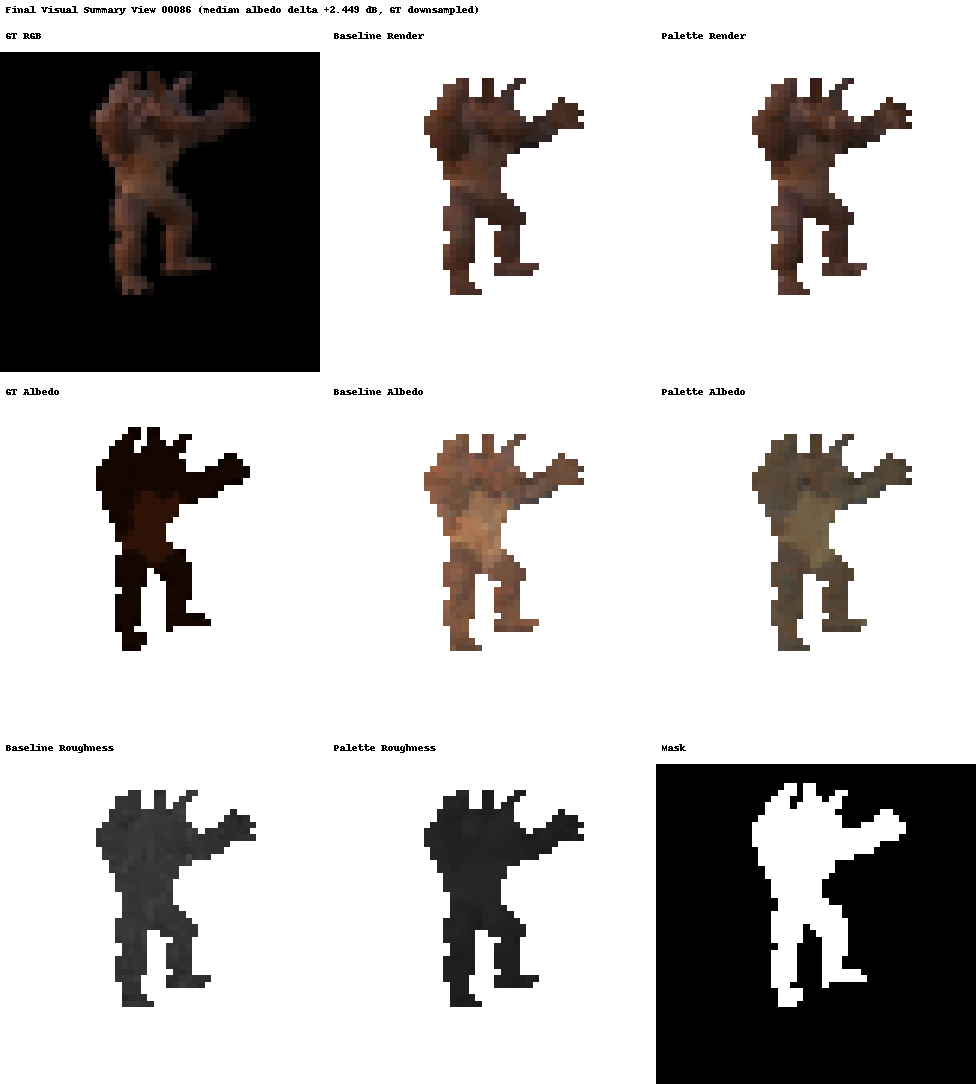
\includegraphics[width=\linewidth]{figure/final_visual_summary.png}
    \caption{Qualitative comparison between non-palette baseline and Palette-Guided. The visualization compares rendered RGB, base color, and roughness results. Palette-Guided produces cleaner and more consistent base color, while the rendered result shows a slight loss in local appearance fitting.}
    \label{fig:palette_guided_visual}
\end{figure}

从图 \ref{fig:palette_guided_visual} 可以进一步观察到，Palette-Guided 的 \texttt{base\_color} 更接近 GT albedo，整体颜色分布更加统一，部分局部明暗残差得到抑制。与此同时，render/PBR 结果中仍能看到一定的细节拟合下降。这说明该方法形成了一个较清晰的 decomposition-vs-fitting trade-off：通过牺牲部分图像重建拟合能力，换取更干净、更可解释的材质分解结果。

总体来看，Palette-Guided 达到了本文 patch 的主要目标。它并不是为了单纯提升训练视角或测试视角的 RGB 重建指标，而是通过共享材质原型约束，改善 SVG-IR 中局部材质参数过于自由所带来的 albedo 分解不一致问题。当前版本的主要不足是 palette 约束仍然较强，导致 PBR 与 NVS 指标下降。后续可以考虑引入 residual gate 或 selective refinement，使模型只在高误差区域释放更多局部材质自由度，从而在保持材质一致性的同时补回局部细节拟合能力。